%!TEX root = Report.tex


\chapter{Working with vector graphics }\label{c:vectorgraphics}

\section{Export Matlab figures}\label{s:matlabfigures}
To achieve good results with Matlab figures in \LaTeX{} they should be exported in a vectorized format such as PDF. Plots can then be scaled without loss of quality which is advantageous when they will be used on a poster for example. Also they can easily be edited using a vector graphics editor such as Inkscape (\url{www.inkscape.org}).

\vspace{5mm}
Adjust font size:
\begin{enumerate}
\item Select \textit{File - Export Setup} from the figure window.
\item Select the \textit{Fonts} tab and enter a fixed font size of 12-14pt.
\item Click \textit{Apply to Figure} to execute the changes.
\end{enumerate}


Click the \textit{Export...} button to export the figure. In the next step select the PDF format and save it.
\vspace{5mm}

It might happen that your small plot is exported in a PDF file in A4 format. 
To adjust the PDF paper size proceed as follows:
\begin{enumerate}
\item Select \textit{File - Export Setup} from the figure window.
\item In the \textit{Size} tab enter the desired dimensions of the figure and click \textit{Apply to Figure} to execute the changes.
\item Don't close the \textit{Export Setup} window and go to \textit{File - Print Preview...}.
\item In \textit{Print Preview } adjust the paper size to the same dimensions already selected in the \textit{Export Setup} .
\item Go back to the \textit{Export Setup} window and click \textit{Export...} to finally save the figure in PDF format. 
\end{enumerate}



Another way to solve this problem is to use a Matlab script which adjusts the paper size to the current figure size and exports it as a PDF file:

% ******************* MATLAB Code *******************
\begin{lstlisting}
function figure2pdf(name)

set(gcf, 'Units', 'centimeters');
pos=get(gcf,'Position');
size=[0 0 pos(3) pos(4)];

% Set the necessary dimensions
set(gcf,'PaperUnits', 'centimeters', 'PaperSize', size(3:4),...
        'PaperPositionMode', 'manual', 'PaperPosition', size,...
        'Renderer', 'painters');
        
% export in PDF format
print(gcf, '-dpdf', [name '.pdf']);
\end{lstlisting}


Note that Matlab code can be illustrated with the mcode package:

\begin{verbatim}
\begin{lstlisting} ...Your Matlab code... \end{lstlisting}
\end{verbatim}


\section{Edit vector graphics}\label{s:editgraphics}
Figures which were exported as shown in section \ref{s:matlabfigures} can easily be edited. Line width, color, style and even shape can be changed and also text can be modified or added.

\begin{figure}[h]
   \centering
   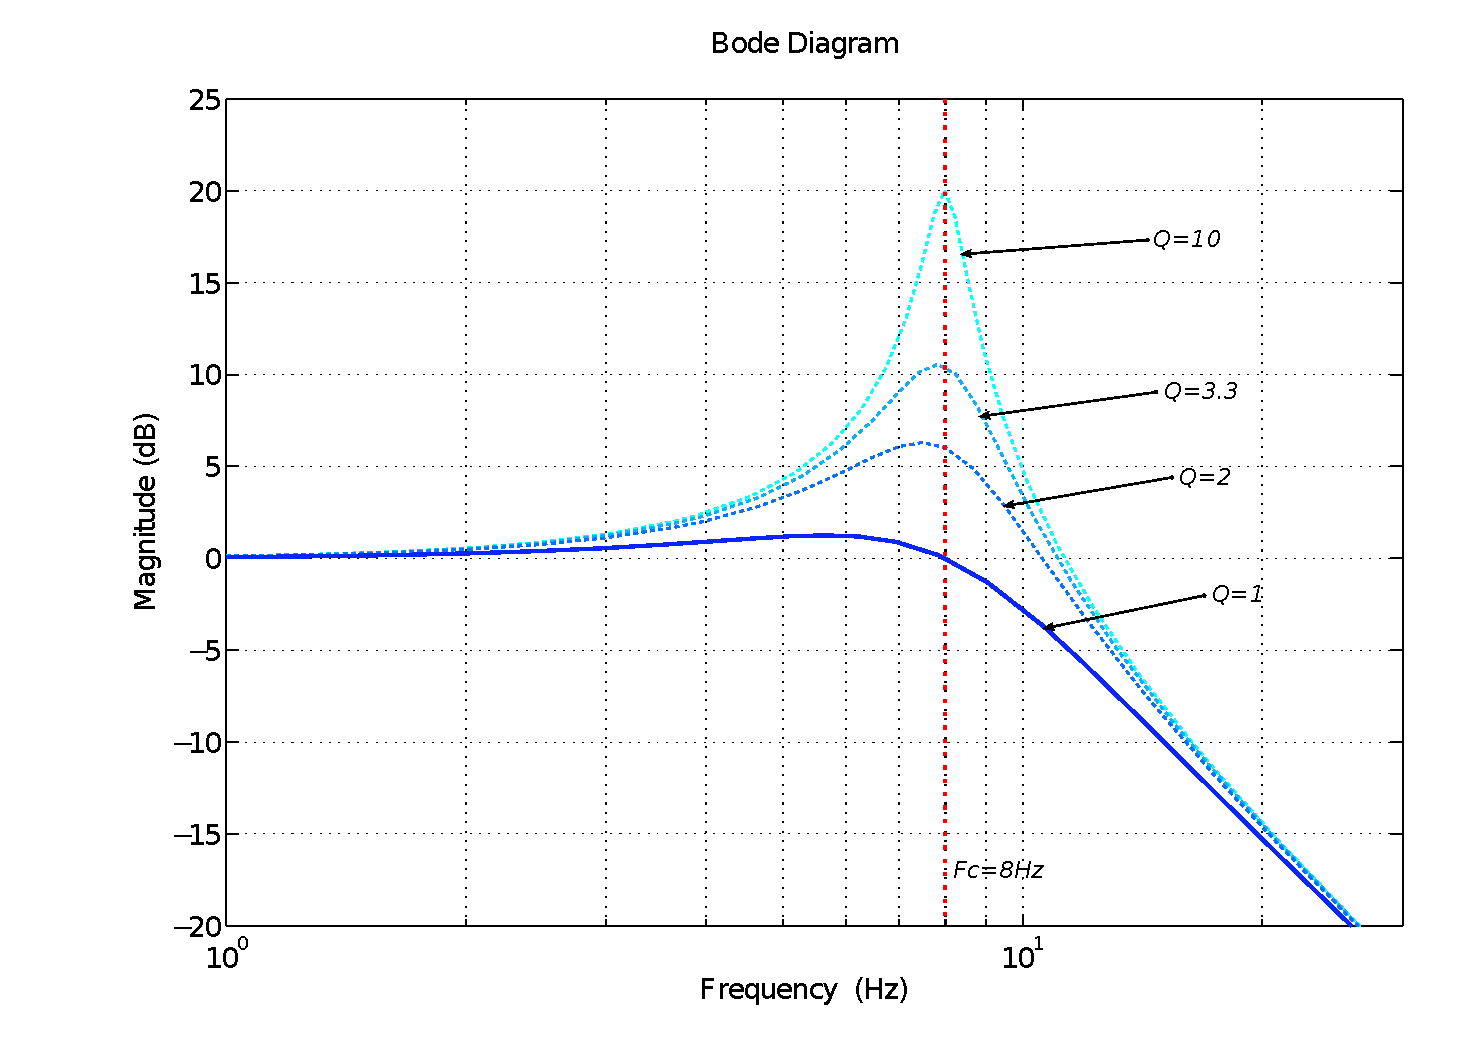
\includegraphics[width=0.8\textwidth]{pics/secondorder_edit.pdf}
   \caption{Bode plot of a second order system with different Q settings.}
   \label{p:secondorder}
\end{figure}

Vector graphics can be combined with bitmap images. This is useful for placing labels in pictures. As this bitmap remains rasterized, it is advantageous to work with resolutions of at least 150dpi if you plan to use the image in a report. 

\newpage

\begin{figure}[h]
   \centering
   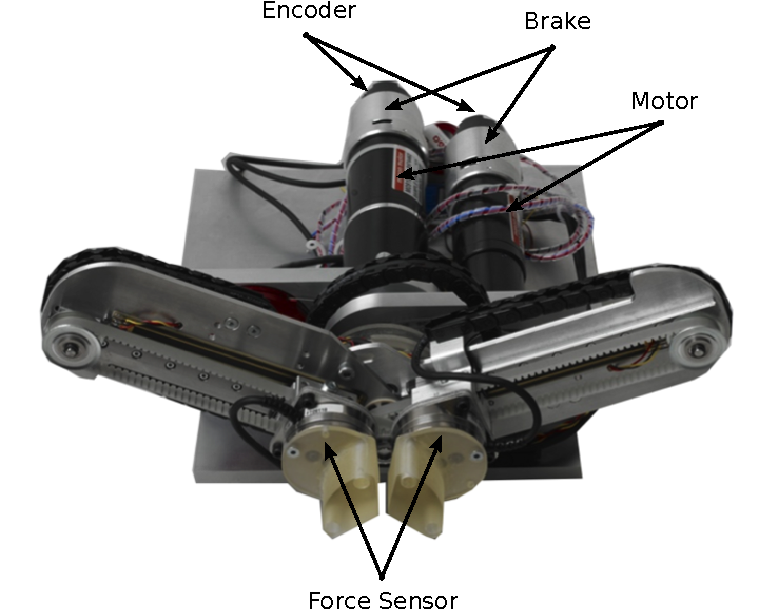
\includegraphics[width=0.8\textwidth]{pics/ReHapticKnob_edit.pdf}
   \caption{A recent version of a hand rehabilitation robot: the ReHapticKnob.}
   \label{p:rehapticknob}
\end{figure}

\vspace{10cm}
